\documentclass[tikz, border=6mm]{standalone}
\begin{document}
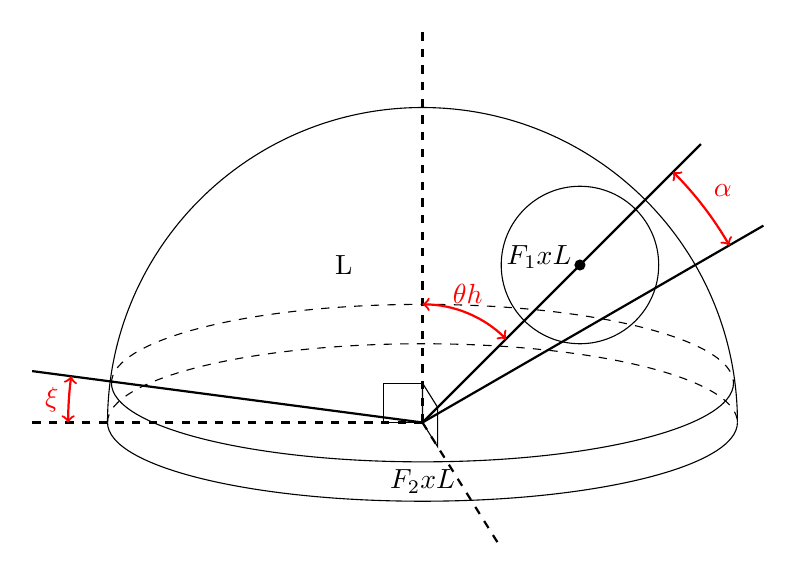
\begin{tikzpicture}
 % base circle
 \draw (-4,0) arc (180:360:4 and 1);
 \draw [dashed] (-4,0) arc (180:0:4 and 1);
 % circle above base circle
 \draw (-3.95,.5) arc (180:360:3.95 and 1);
 \draw [dashed] (-3.95,.5) arc (180:0:3.95 and 1);
 % hemisphere
 \draw (-4,0) arc (180:0:4 and 4);
 % circle on hemisphere and point in it
 \draw (2,2) circle (1);
 \draw (2,2) node [circle, fill=black, inner sep=.05cm, label={[label distance=-.25cm]95:$F_1xL$}] (dot) {};
 % rectangles at zero
 \draw (0,0,0) -- ++(0,-.5,-.5) -- ++(0,.5,0) -- ++(0,.5,.5) -- cycle;
 \draw (0,0) -- ++(-.5,0) -- ++(0,.5) -- ++(.5,0) -- cycle;
 % x and spanning xi
 \draw [thick, dashed] (0,0) -- ++(-5,0);
 \draw [thick] (0,0) -- ++(172.5:5cm);
 % y
 \draw [thick, dashed] (0,0) -- ++(0,5);
 % z
 \draw [thick, dashed] (0,0,0) -- ++(0,-2.5,-2.5);
 % lines spanning angle alpha
 \draw [thick] (0,0) -- ++(45:5cm);
 \draw [thick] (0,0) -- ++(30:5cm);
 % angle labels
 \draw [red, thick, <->] (0,0) ++(172.5:4.5cm) arc (172.5:180:4.5cm) node [midway, left] () {$\xi$};
 \draw [red, thick, <->] (0,0) ++(30:4.5cm) arc (30:45:4.5cm) node [midway, above right] () {$\alpha$};  
 \draw [red, thick, <->] (0,0) ++(90:1.5cm) arc (90:45:1.5cm) node [midway, above] () {$\theta h$};
 % other labels
 \draw (0,-.75) node () {$F_2xL$};
 \draw (-1,2) node () {L};
\end{tikzpicture}
\end{document}